\begin{frame}{Edge inference on DREAM networks - 10 nodes}
\label{sec:dream_results}
\begin{columns}
\begin{column}{0.4\textwidth}
% The DREAM data goldstandards for the five 10-node graphs were used for simulation of node values using the simple iteration method~(\autoref{sec:prim}), after randomly assigning uniform edge strengths in range~$[-1,1]$.

\begin{figure}[ht]
    \centering
    \includegraphics[width=\textwidth]{analysis/fig/edge_cor_10.pdf}
    \caption{\textbf{Predicted vs. true edge values.} 5 10-node networks. Simple simulation. }
    \label{fig:edge_value_cor_10}
\end{figure}

% The resulting inferred edge values for a single edge inference attempt on each graph are compared to the true edge values~(\autoref{fig:edge_value_cor_10}). There are three undetectable edges for the five graphs. They are included in this plot and all have a score of zero. The points along the line \texttt{score}=\texttt{true} are edges where the weight~(score) accurately predicts the true edge strength used for node value simulation. A few outlier protein kinase edges can be seen as being misclassified. Most values are found in the point (0,0) which are all non-edges correctly classfied as non-edges (true negatives). The purpose of the plot is to show that for very simple cases the edges are not only found, but their exact edge value is also inferred. It also shows that there is 1 false positive and 1 false negative of the 15 detectable PK edges, and that inference on TF edges are perfect in this simple example.
\begin{itemize}
    \item Predicted edge values accurate to truth
    \item LLC fails for kinases
\end{itemize}
\end{column}
\begin{column}{0.6\textwidth}

\begin{figure}[ht]
\centering
\begin{subfigure}[b]{0.49\textwidth}\centering\caption{}
\includegraphics[width=\textwidth]{analysis/fig/roc_pk_10.pdf}
\end{subfigure}
\hfill
\begin{subfigure}[b]{0.49\textwidth}\centering\caption{}
\includegraphics[width=\textwidth]{analysis/fig/roc_pk_llc_10.pdf}
\end{subfigure}
\caption{\textbf{ROC curves for 5 10-node networks.} $\boldsymbol{e}$-minimization~(a) and LLC~\cite{EberhardtLLC}~(b) on PK edges. neg: inference of negative edges, pos: positive, abs: ignoring sign. AUCs are micro averaged.}
\label{fig:roc_pk_10}
\end{figure}

% The inference can also be described with ROC curves for outgoing PK edges in each individual graph~(\autoref{fig:roc_pk_10}). Inference of the presence or absence of edges from transcription factors to genes were perfect on this simple simulation~(AUC=1). For protein kinases the inference is less trivial, as we see that AUCs drops below perfect scores. Note that most curves are perfect, and that the ones not following the path (0,0)$\rightarrow$(0,1)$\rightarrow$(1,1) are a minority. This is also apparent from the AUC scores, which are close to perfect. The ROC curves are also shown for inference performed using the LLC method~\cite{EberhardtLLC}. Since it infers linear direct causal interactions and it fails to classify presence and absence of outgoing PK edges based on their indirect effects on the observed node values.
\end{column}
\end{columns}
\end{frame}

\begin{frame}{Edge inference on DREAM networks - 100 nodes}
% This comparison is biased towards the equilibrium method since the data simulation is performed with the same equations that are used for the $\boldsymbol{e}$-minimization inference, so to increase realism and fairness of performance testing we move on to the larger 100-node graphs where we will use the more realistic GeneNetWeaver kinase extension code for simulation of observable node values.
\begin{figure}[ht]
\centering
\begin{subfigure}[b]{0.24\textwidth}\centering\caption{}
\includegraphics[width=\textwidth]{analysis/fig/roc_pk_prim.pdf}
\end{subfigure}
\hfill
\begin{subfigure}[b]{0.24\textwidth}\centering\caption{}
\includegraphics[width=\textwidth]{analysis/fig/roc_pk_prim_B.pdf}
\end{subfigure}
\hfill
\begin{subfigure}[b]{0.24\textwidth}\centering\caption{}
\includegraphics[width=\textwidth]{analysis/fig/roc_pk_gnw_pos.pdf}\label{fig:micro_average.c}
\end{subfigure}
\hfill
\begin{subfigure}[b]{0.24\textwidth}\centering\caption{}
\includegraphics[width=\textwidth]{analysis/fig/roc_pk_gnw.pdf}\label{fig:micro_average.d}
\end{subfigure}
\caption{\textbf{ROC curves for PK edge inference.} $\boldsymbol{e}$-minimization~(a,c,d) and $B$-method~(b). Simple simulation~(a,b), and GeneNetWeaver extension~(c,d). True PK edges all positive~(c) or signed~(d). neg: inference on negative edges. pos: positive. abs: ignoring sign. avg: score = avg. $w$ from 20 runs. avg/std: score = avg./std. $w$, other: score = $w$. }
\label{fig:micro_average}
\end{figure}
$\ge 80 \%$ most prominent edges inferred perfectly
% Edge inference was tested on the five 100-node graphs from DREAM4. The simulations were either performed using the simple iteration method~(\autoref{sec:prim}) or the GeneNetWeaver kinase extension method~(\autoref{sec:gnw_extension}). TF inference was almost perfect with AUC=0.992 for detection of presence or absence of edge, which can be seen in the appendix~(\autoref{fig:gnw_each.a}). The ROC curves, shown in~\autoref{fig:micro_average}, are evaluated on comparisons of inferred and true edges, combined of all five graphs~(microaverage). Individual graphs for individual runs can be seen in~\autoref{app:roc} with equivalent AUC scores.
% Data created with the GNW extension were either simulated where true outgoing PK edges were restricted to a uniform distribution with range~$[0,1]$, or without sign restriction. ROC curves for performance of inference on the former is in~\autoref{fig:micro_average.c}, and the latter in~\autoref{fig:micro_average.d}. The reason for restricting the kinase interaction to positive values are based on the kinase model of regulation~(\autoref{sec:gnw_extension}), which builds on a model of phosphorylation regulation involving only protein kinases with positive interactions~(\autoref{sec:Heinrich}). From the ROC curves it is clear that allowing negative outgoing protein kinase edges does not seem to worsen performance of inference. The negative outgoing protein kinase edges can be seen as a dephosphorylation of the target protein, since $\phi_i$ and $y_i$ from~\autoref{sec:gnw_extension} describes phosphorylation values, and not a general activity concept. It shows that the simulation code and method is robust in allowing for dephosphorylation interactions between specific proteins, rather than only as a background decay~$\lambda_i^{(\text{Phos})}$, since the simulations managed to reach approximate convergence and produce similar inference performance to the trials with sign restriction. Phosphatases are often considered as a background effect to let signals decay, due to their low interaction specificity compared to protein kinases. In spite of this, it is useful that direct dephosphorylation can be simulated and inferred since some of the knockouts in the RNA data are phosphatases~(\autoref{sec:yeast_data}).


% The ROC curves shows a quantitative measure of performance but does not show a final inferred network. To select specific edges we choose a threshold. The threshold was chosen as 0.01 which corresponds to approximately accepting 50\% of inferred PK edges across the five graphs with the highet scores, which corresponds to a cutoff at TPR=0.5 in~\autoref{fig:micro_average.c}. The threshold was applied to all five graphs for all edge types, although different threshold for each were found to be optimal. The inferred edges are shown on the graphs~(\autoref{fig:dream_100_infer}). Activation and repression is not indicated, which is the sign of edges from transcription factors. Edges from protein kinases are all activating as per the restriction to elicit phosphorylation and not dephosphorylation. Kinases not connected to any nodes are included next to each graph. The unconnected kinases are the undetectable kinases. The count of undetectable kinases for each graph is 30 minus the "detectable PK nodes" counts listed in~\autoref{tab:dream_data}, since each graph were initially assigned 30 kinases.

% From the plots we get an impression of the intricacy arising from less than 100 nodes. We see that edges inferred can often be trusted, detects many of the true edges, and that false positives for PK edges arises in situations where there would be ambiguity in what regulation to expect, given only the relative gene expressions. An example is the $\text{PK}_{14}\rightarrow\text{PK}_{29}$ edge at the top-right of net 100.4.
\end{frame}

\begin{frame}{Edge inference on DREAM networks - 100 nodes}
\begin{figure}[ht]
    \centering
    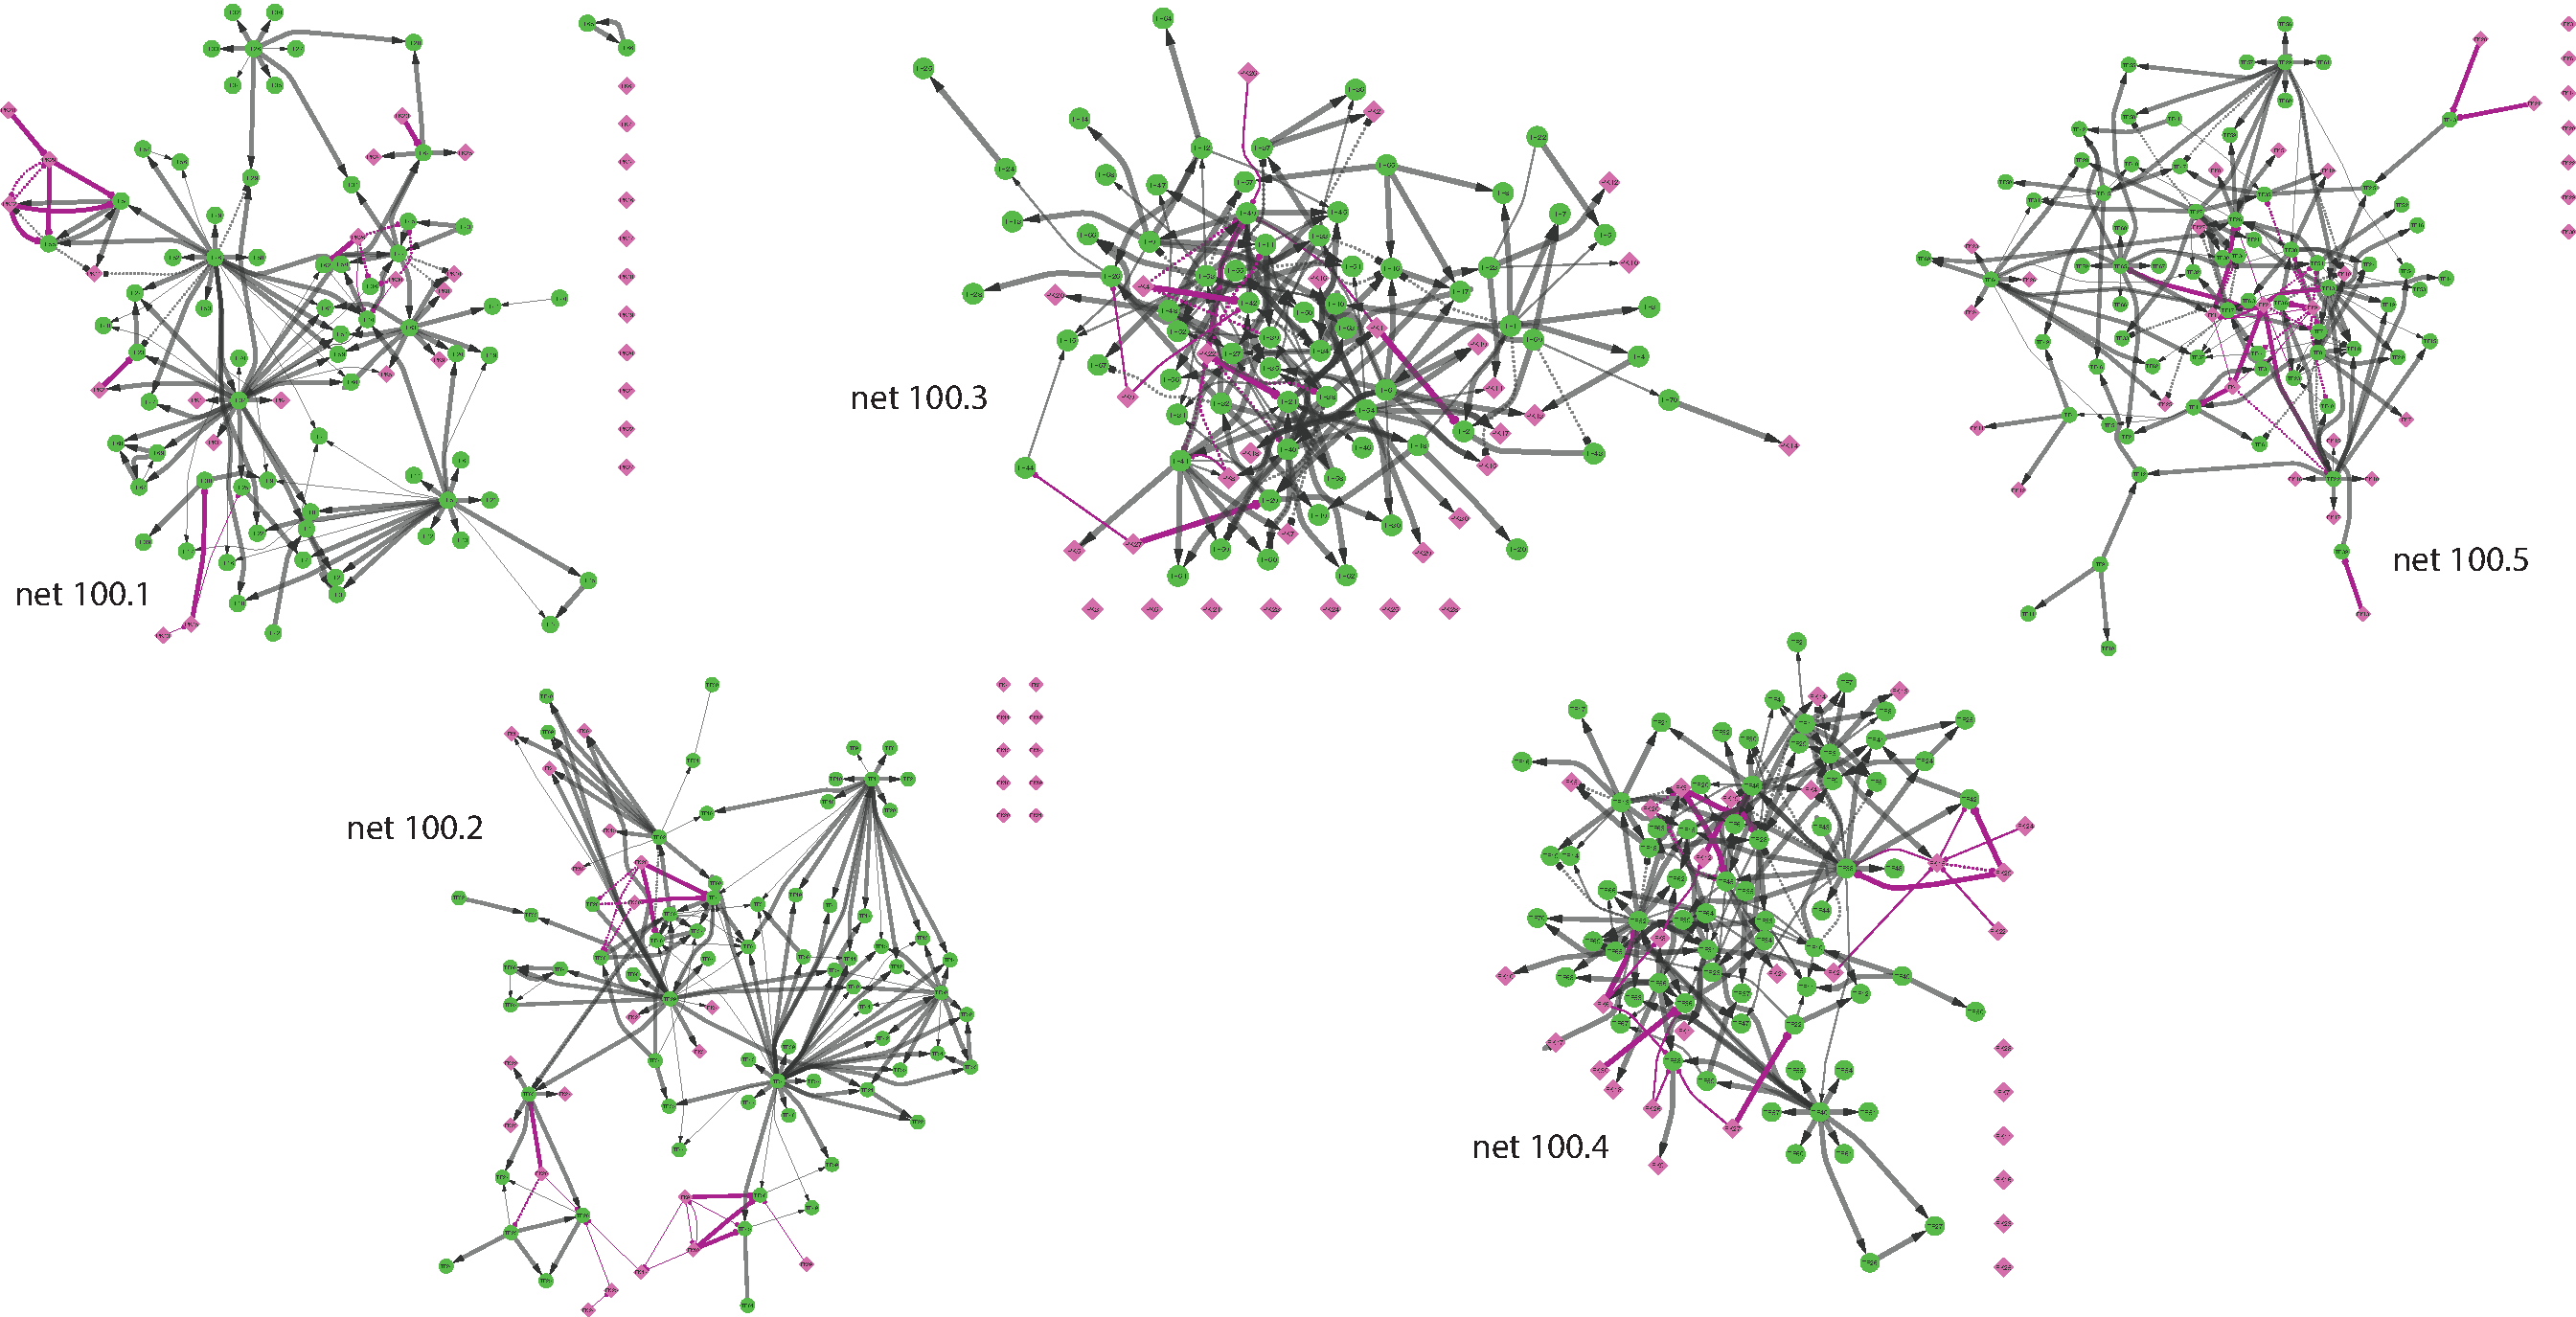
\includegraphics[width=.93\textwidth]{analysis/fig/dream100_infer_pres.pdf}
    \caption{\textbf{Inferred edges of 5 100-node networks.} Edge inferred from single $\boldsymbol{e}$-minimization when $w>0.01$. \textbf{Thick line} = TP, thin = FN, dotted = FP, none = TN. \textcolor{gray}{Dim line} = TF edge, \textcolor{pk!50!magenta}{magenta} = PK edge. }
    \label{fig:dream_100_infer}
\end{figure}
\end{frame}

